\documentclass[12pt,a4paper]{article}
\usepackage{amsfonts}
\usepackage{amsmath}
\usepackage{amssymb}
\usepackage{graphicx}
\usepackage[left=2cm,right=2cm,top=2cm,bottom=2cm]{geometry}
\usepackage{tikz}
\usepackage{pgfplots}

\author{Sarvesh Subramaniam M}
\title{Multipole Expansion in Electrostatics and Magnetostatics}
\date{June 9,2023}
\begin{document}

\maketitle
\section{CH22B009}
\subsection{Introduction}
In physics, spherical multipole moments are the coefficients in a series expansion of a potential that varies inversely with the distance R to a source
\subsection{Multipole Expansion Equation in Electrostatics}
\begin{equation}
V(\mathbf{r}) = \frac{1}{4\pi\epsilon_0} \sum_{n=0}^{\infty} \frac{1}{r^{n+1}} \int r^{n} P_l(\cos(\alpha)) \rho(\mathbf{r}')\, d(\tau')\footnote{Introduction To Electrodynamics by David J. Griffiths,4th Edition}
\end{equation}
$\alpha$ = angle between r - r' and r'\\
$\sum$ = summation\\
$\int$ = integral\\
$\rho$ = charge density of source \\
$\tau$ = small volume element \\
$V$ = potential \\
$r$ = distance from origin \\
$r'$ = distance from source \\
$\epsilon_0$ = permittivity of free space \\
$P_l$ = Legendre Polynomial \\
A multipole expansion is a mathematical series representing a function that depends on angles—usually the two angles on a sphere. These series are useful because they can often be truncated, meaning that only the first few terms need to be retained for a good approximation to the original function. Multipole expansions are very frequently used in the study of electromagnetic and gravitational fields, where the fields at distant points are given in terms of sources in a small region. The multipole expansion with angles is often combined with an expansion in radius. Such a combination gives an expansion describing a function throughout three-dimensional space.

The multipole expansion is expressed as a sum of terms with progressively finer angular features. For example, the initial term—called the zeroth, or monopole, moment—is a constant, independent of angle. The following term—the first, or dipole, moment—varies once from positive to negative around the sphere. Higher-order terms (like the quadrupole and octupole) vary more quickly with angles. A multipole moment usually involves powers (or inverse powers) of the distance to the origin, as well as some angular dependence.
\subsection{plot for multipole expansion in electrostatics}
\subsubsection{$\frac{Q}{4\pi\epsilon_0} = 1$}
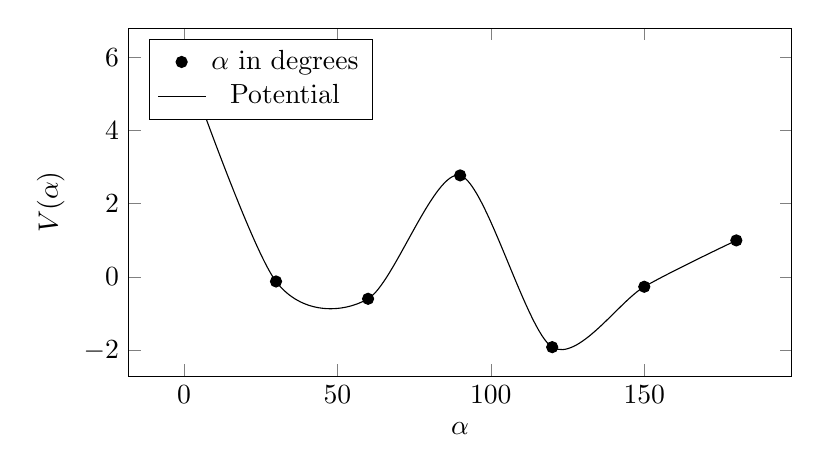
\begin{tikzpicture}
  \begin{axis}[
    xlabel={$\alpha$},
    ylabel={$V(\alpha)$},
    legend pos=north west,
    width=10cm,
    height=6cm
  ]
    
    \addplot [only marks] coordinates {
      (0, 6)
      (30, 	-0.1208104538)
      (60, 	-0.5941090091)
      (90,	2.774402376)
      (120, 	-1.9138129113)
      (150, -0.2649856493)
      (180, 1)
    };
    
    \addplot [smooth] coordinates {
      (0, 6)
      (30, 	-0.1208104538)
      (60, 	-0.5941090091)
      (90,	2.774402376)
      (120, 	-1.9138129113)
      (150, -0.2649856493)
      (180, 1)
    };
    
    \legend{$\alpha$ in degrees, Potential}
  \end{axis}
\end{tikzpicture} \\

\subsection{Multipole expansion in Magnetostatics}
\begin{equation}
A(\mathbf{r}) = \frac{\mu_0I}{4\pi} \sum_{n=0}^{\infty} \frac{1}{r^{n+1}} \oint r^{n} P_l(\cos(\alpha))d(\mathbf{l}') 
\end{equation}
$\alpha$ = angle between r - r' and r'\\
$\sum$ = summation\\
$\int$ = integral\\
$A$ = Vector Potential\\
$r$ = distance from origin \\
$I$ = current\\
$\mathbf{l}'$ = small current element\\
$P_l$ = Legendre Polynomial \\
$\mu_0$ = permeability of free space\\
The magnetic multipole expansion is an analogous concept to the electrostatic multipole expansion, but it applies to the magnetic field instead of the electric field. It allows us to express the magnetic field in terms of magnetic moments of various orders. Similar to the electrostatic case, the magnetic multipole expansion provides a way to approximate the magnetic field in situations where the sources of the field have complex distributions.

The magnetic multipole expansion is typically expressed in terms of vector spherical harmonics, which are the magnetic analogs of the scalar spherical harmonics used in the electrostatic case. These vector spherical harmonics describe the spatial dependence of the magnetic field.

\subsection{plot for magnetic multipole expansion}
\subsubsection{$\mu_0\frac{I}{4\pi} = 1$}
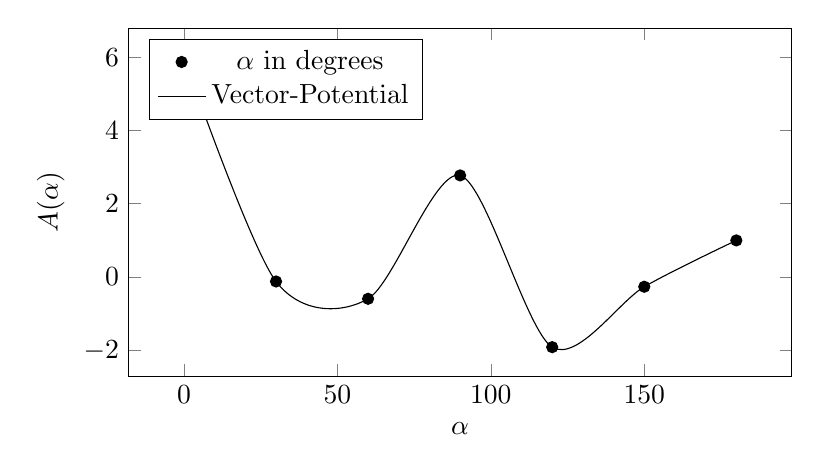
\begin{tikzpicture}
  \begin{axis}[
    xlabel={$\alpha$},
    ylabel={$A(\alpha)$},
    legend pos=north west,
    width=10cm,
    height=6cm
  ]
    
    \addplot [only marks] coordinates {
      (0, 6)
      (30, 	-0.1208104538)
      (60, 	-0.5941090091)
      (90,	2.774402376)
      (120, 	-1.9138129113)
      (150, -0.2649856493)
      (180, 1)
    };
   
    \addplot [smooth] coordinates {
      (0, 6)
      (30, 	-0.1208104538)
      (60, 	-0.5941090091)
      (90,	2.774402376)
      (120, 	-1.9138129113)
      (150, -0.2649856493)
      (180, 1)
    };
    
    \legend{$\alpha$ in degrees, Vector-Potential}
  \end{axis}
\end{tikzpicture}


\section{github user name and name}
Name:Sarvesh Subramaniam M \\
Github user name:Sarvesh528491\\



\end{document}